\documentclass[10pt, sigplan]{acmart}
\usepackage[utf8]{inputenc}
\usepackage[T1]{fontenc}

\newcommand{\packageGraphicx}{\usepackage{graphicx}}
\newcommand{\packageHyperref}{\usepackage{hyperref}}
\newcommand{\renewrmdefault}{\renewcommand{\rmdefault}{ptm}}
\newcommand{\packageRelsize}{\usepackage{relsize}}
% amsmath is required for the combination of {mathabx,
% wasysym, newtxmath} to work. Otherwise, newtxmath
% would load amsmath *after* mathabx and wasysym,
% causing command redefinition issues.
\newcommand{\packageAmsmath}{\usepackage{amsmath}}
\newcommand{\packageMathabx}{\usepackage{mathabx}}
% Avoid conflicts between "mathabx" and "wasysym",
% and between "wasysym" integrals and "amsmath" integrals (iint).
\newcommand{\packageWasysym}{
  \let\leftmoon\relax \let\rightmoon\relax \let\fullmoon\relax \let\newmoon\relax \let\diameter\relax
  \usepackage[nointegrals]{wasysym}}
% Both newtxmath and mathabx define the \widering command.
% The only reason we choose the newtxmath version is that
% acmart.cls is also using the one from newtxmath.
\newcommand{\packageTxfonts}{
  \let\widering\relax
  \let\oldwidebar\widebar
  \let\widebar\relax
  \usepackage{newtxmath}
  % if newtxmath is before version 1.7.0,
  % then we are still going to use widebar from mathabx
  \ifx\widebar\relax
    \let\widebar\oldwidebar
  \fi
}
\newcommand{\packageTextcomp}{\usepackage{textcomp}}
\newcommand{\packageFramed}{\usepackage{framed}}
\newcommand{\packageHyphenat}{\usepackage[htt]{hyphenat}}
\newcommand{\packageColor}{\usepackage[usenames,dvipsnames]{color}}
\newcommand{\doHypersetup}{\hypersetup{bookmarks=true,bookmarksopen=true,bookmarksnumbered=true}}
\newcommand{\packageTocstyle}{}
\newcommand{\packageCJK}{\IfFileExists{CJK.sty}{\usepackage{CJK}}{}}
%%%%%%%%%%%%%%%%%%%%%%%%%%%%%%%%%%%%%%%%%%%%%%%%%%%%%%%%%%%%%%%%%%%%%%%%%%%%%%%%
% BEGIN acmart-load.tex
% Avoid package option conflict
\renewcommand\packageColor\relax
\renewcommand\packageTocstyle\relax
\renewcommand\packageMathabx{\ifx\bigtimes\undefined \usepackage{mathabx} \else \relax \fi}
% Both 'mathabx' and 'newtxmath' (required by the 'acmart' class) define a '\bigtimes' command. 
\renewcommand\packageTxfonts\relax
\let\Footnote\undefined
\let\captionwidth\undefined
\renewcommand{\renewrmdefault}{}
% END acmart-load.tex
%%%%%%%%%%%%%%%%%%%%%%%%%%%%%%%%%%%%%%%%%%%%%%%%%%%%%%%%%%%%%%%%%%%%%%%%%%%%%%%%
% This is the default style configuration for Scribble-generated Latex

\packageGraphicx
\packageHyperref
\renewrmdefault
\packageRelsize
\packageAmsmath
\packageMathabx
\packageWasysym
\packageTxfonts
\packageTextcomp
\packageFramed
\packageHyphenat
\packageColor
\doHypersetup
\packageTocstyle
\packageCJK


%%%%%%%%%%%%%%%%%%%%%%%%%%%%%%%%%%%%%%%%%%%%%%%%%%%%%%%%%%%%%%%%%%%%%%%%%%%%%%%%
% Configuration that is especially meant to be overridden:

% Inserted before every ``chapter'', useful for starting each one on a new page:
\newcommand{\sectionNewpage}{}
% Inserted before every book ``part''
\newcommand{\partNewpage}{\sectionNewpage}

% Hooks for actions within the `document' environment:
\newcommand{\preDoc}{}
\newcommand{\postDoc}{}

% Generated by `secref'; first arg is section number, second is section title:
\newcommand{\BookRef}[2]{\emph{#2}}
\newcommand{\ChapRef}[2]{\SecRef{#1}{#2}}
\newcommand{\SecRef}[2]{section~#1}
\newcommand{\PartRef}[2]{part~#1}
% Generated by `Secref':
\newcommand{\BookRefUC}[2]{\BookRef{#1}{#2}}
\newcommand{\ChapRefUC}[2]{\SecRefUC{#1}{#2}}
\newcommand{\SecRefUC}[2]{Section~#1}
\newcommand{\PartRefUC}[2]{Part~#1}

% Variants of the above with a label for an internal reference:
\newcommand{\BookRefLocal}[3]{\hyperref[#1]{\BookRef{#2}{#3}}}
\newcommand{\ChapRefLocal}[3]{\hyperref[#1]{\ChapRef{#2}{#3}}}
\newcommand{\SecRefLocal}[3]{\hyperref[#1]{\SecRef{#2}{#3}}}
\newcommand{\PartRefLocal}[3]{\hyperref[#1]{\PartRef{#2}{#3}}}
\newcommand{\BookRefLocalUC}[3]{\hyperref[#1]{\BookRefUC{#2}{#3}}}
\newcommand{\ChapRefLocalUC}[3]{\hyperref[#1]{\ChapRefUC{#2}{#3}}}
\newcommand{\SecRefLocalUC}[3]{\hyperref[#1]{\SecRefUC{#2}{#3}}}
\newcommand{\PartRefLocalUC}[3]{\hyperref[#1]{\PartRefUC{#2}{#3}}}

% Variants of the above with a section number is empty (i.e., UnNumbered):
\newcommand{\BookRefUN}[1]{\BookRef{}{#1}}
\newcommand{\ChapRefUN}[1]{\SecRefUN{#1}}
\newcommand{\SecRefUN}[1]{``#1''}
\newcommand{\PartRefUN}[1]{\SecRefUN{#1}}
\newcommand{\BookRefUCUN}[1]{\BookRefUN{#1}}
\newcommand{\ChapRefUCUN}[1]{\ChapRefUN{#1}}
\newcommand{\SecRefUCUN}[1]{\SecRefUN{#1}}
\newcommand{\PartRefUCUN}[1]{\PartRefUN{#1}}

\newcommand{\BookRefLocalUN}[2]{\hyperref[#1]{\BookRefUN{#2}}}
\newcommand{\ChapRefLocalUN}[2]{\SecRefLocalUN{#1}{#2}}
\newcommand{\SecRefLocalUN}[2]{\hyperref[#1]{\SecRefUN{#2}}}
\newcommand{\PartRefLocalUN}[2]{\SecRefLocalUN{#1}{#2}}
\newcommand{\BookRefLocalUCUN}[2]{\BookRefLocalUN{#1}{#2}}
\newcommand{\ChapRefLocalUCUN}[2]{\ChapRefLocalUN{#1}{#2}}
\newcommand{\SecRefLocalUCUN}[2]{\SecRefLocalUN{#1}{#2}}
\newcommand{\PartRefLocalUCUN}[2]{\PartRefLocalUN{#1}{#2}}

\newcommand{\SectionNumberLink}[2]{\hyperref[#1]{#2}}

% Enabled with a 'enable-index-merge part style property. This default
% implementation isn't good enough, because the argument is a
% comma-separated sequence of labels:
\newcommand{\Smanypageref}[1]{\pageref{#1}}

%%%%%%%%%%%%%%%%%%%%%%%%%%%%%%%%%%%%%%%%%%%%%%%%%%%%%%%%%%%%%%%%%%%%%%%%%%%%%%%%
% Fonts

% Font commands used by generated text:
\newcommand{\Scribtexttt}[1]{{\texttt{#1}}}
\newcommand{\textsub}[1]{$_{\hbox{\textsmaller{#1}}}$}
\newcommand{\textsuper}[1]{$^{\hbox{\textsmaller{#1}}}$}
\newcommand{\intextcolor}[2]{\textcolor{#1}{#2}}
\newcommand{\intextrgbcolor}[2]{\textcolor[rgb]{#1}{#2}}
\newcommand{\incolorbox}[2]{{\fboxrule=0pt\fboxsep=0pt\protect\colorbox{#1}{#2}}}
\newcommand{\inrgbcolorbox}[2]{{\fboxrule=0pt\fboxsep=0pt\protect\colorbox[rgb]{#1}{#2}}}
\newcommand{\plainlink}[1]{#1}
\newcommand{\techoutside}[1]{#1}
\newcommand{\techinside}[1]{#1}
\newcommand{\badlink}[1]{#1}
\newcommand{\indexlink}[1]{#1}
\newcommand{\noborder}[1]{#1}
\newcommand{\Smaller}[1]{\textsmaller{#1}}
\newcommand{\Larger}[1]{\textlarger{#1}}
\newcommand{\planetName}[1]{PLane\hspace{-0.1ex}T}
\newcommand{\slant}[1]{{\textsl{#1}}}

% Used for <, >, and | in tt mode. For some fonts and installations,
% there seems to be an encoding issue, so pick T1 explicitly:
\newcommand{\Stttextmore}{{\fontencoding{T1}\selectfont>}}
\newcommand{\Stttextless}{{\fontencoding{T1}\selectfont<}}
\newcommand{\Stttextbar}{{\fontencoding{T1}\selectfont|}}

%%%%%%%%%%%%%%%%%%%%%%%%%%%%%%%%%%%%%%%%%%%%%%%%%%%%%%%%%%%%%%%%%%%%%%%%%%%%%%%%
% Tables

% The `stabular' environment seems to be the lesser of evils among 
%  page-breaking table environments (and we've made a copy as ``pltstabular'
%  to make sure that it doesn't change).

\makeatletter
%%%%%%%%%%%%%%%%%%%%%%%%%%%%%%%%%%%%%%%%%%%%%%%%%%%%%%%%%%%%%%%%%%%%%%
\message{pltstabular is a modification of stabular}
%% A renamed version of:
%% stabular.sty
%% Copyright 1998 Sigitas Tolu\v sis
%% VTeX Ltd., Akademijos 4, Vilnius, Lithuania
%% e-mail sigitas@vtex.lt
%% http://www.vtex.lt/tex/download/macros/
%%
% This program can redistributed and/or modified under the terms
% of the LaTeX Project Public License Distributed from CTAN
% archives in directory macros/latex/base/lppl.txt; either
% version 1 of the License, or (at your option) any later version.
%
% PURPOSE:   Improve tabular environment.
%
% SHORT DESCRIPTION:
%
% Changed internal commands: \@mkpream, \@addamp, \@xhline
%
% Provides new commands in tabular (used after command \\):
% \emptyrow[#1] 
% -------------
%    Adds empty row, #1 - height of the row 
%
% \tabrow{#1}[#2] 
% ---------------
%    Adds row of natural height: #1\\[#2]
%
% Provides new environments: pltstabular and pltstabular* 
%                            --------     ---------
%            One more multi-page version of tabular
%
%
\def\empty@finalstrut#1{%
  \unskip\ifhmode\nobreak\fi\vrule\@width\z@\@height\z@\@depth\z@}
\def\no@strut{\global\setbox\@arstrutbox\hbox{%
    \vrule \@height\z@
           \@depth\z@
           \@width\z@}%
    \gdef\@endpbox{\empty@finalstrut\@arstrutbox\par\egroup\hfil}%
}%
\def\yes@strut{\global\setbox\@arstrutbox\hbox{%
    \vrule \@height\arraystretch \ht\strutbox
           \@depth\arraystretch \dp\strutbox
           \@width\z@}%
    \gdef\@endpbox{\@finalstrut\@arstrutbox\par\egroup\hfil}%
}%
\def\@mkpream#1{\@firstamptrue\@lastchclass6
  \let\@preamble\@empty\def\empty@preamble{\add@ins}%
  \let\protect\@unexpandable@protect
  \let\@sharp\relax\let\add@ins\relax
  \let\@startpbox\relax\let\@endpbox\relax
  \@expast{#1}%
  \expandafter\@tfor \expandafter
    \@nextchar \expandafter:\expandafter=\reserved@a\do
       {\@testpach\@nextchar
    \ifcase \@chclass \@classz \or \@classi \or \@classii \or \@classiii
      \or \@classiv \or\@classv \fi\@lastchclass\@chclass}%
  \ifcase \@lastchclass \@acol
      \or \or \@preamerr \@ne\or \@preamerr \tw@\or \or \@acol \fi}
\def\@addamp{%
  \if@firstamp
    \@firstampfalse
    \edef\empty@preamble{\add@ins}%
  \else
    \edef\@preamble{\@preamble &}%
    \edef\empty@preamble{\expandafter\noexpand\empty@preamble &\add@ins}%
  \fi}
\newif\iftw@hlines \tw@hlinesfalse
\def\@xhline{\ifx\reserved@a\hline
               \tw@hlinestrue
             \else\ifx\reserved@a\Hline
               \tw@hlinestrue
             \else
               \tw@hlinesfalse
             \fi\fi
      \iftw@hlines
        \aftergroup\do@after
      \fi
      \ifnum0=`{\fi}%
}
\def\do@after{\emptyrow[\the\doublerulesep]}
\def\emptyrow{\noalign\bgroup\@ifnextchar[\@emptyrow{\@emptyrow[\z@]}}
\def\@emptyrow[#1]{\no@strut\gdef\add@ins{\vrule \@height\z@ \@depth#1 \@width\z@}\egroup%
\empty@preamble\\
\noalign{\yes@strut\gdef\add@ins{\vrule \@height\z@ \@depth\z@ \@width\z@}}%
}
\def\tabrow#1{\noalign\bgroup\@ifnextchar[{\@tabrow{#1}}{\@tabrow{#1}[]}}
\def\@tabrow#1[#2]{\no@strut\egroup#1\ifx.#2.\\\else\\[#2]\fi\noalign{\yes@strut}}
%
\def\endpltstabular{\crcr\egroup\egroup \egroup}
\expandafter \let \csname endpltstabular*\endcsname = \endpltstabular
\def\pltstabular{\let\@halignto\@empty\@pltstabular}
\@namedef{pltstabular*}#1{\def\@halignto{to#1}\@pltstabular}
\def\@pltstabular{\leavevmode \bgroup \let\@acol\@tabacol
   \let\@classz\@tabclassz
   \let\@classiv\@tabclassiv \let\\\@tabularcr\@stabarray}
\def\@stabarray{\m@th\@ifnextchar[\@sarray{\@sarray[c]}}
\def\@sarray[#1]#2{%
  \bgroup
  \setbox\@arstrutbox\hbox{%
    \vrule \@height\arraystretch\ht\strutbox
           \@depth\arraystretch \dp\strutbox
           \@width\z@}%
  \@mkpream{#2}%
  \edef\@preamble{%
    \ialign \noexpand\@halignto
      \bgroup \@arstrut \@preamble \tabskip\z@skip \cr}%
  \let\@startpbox\@@startpbox \let\@endpbox\@@endpbox
  \let\tabularnewline\\%
%    \let\par\@empty
    \let\@sharp##%
    \set@typeset@protect
    \lineskip\z@skip\baselineskip\z@skip
    \@preamble}

%%%%%%%%%%%%%%%%%%%%%%%%%%%%%%%%%%%%%%%%%%%%%%%%%%%%%%%%%%%%%%%%%%%%%%
\makeatother

\newenvironment{bigtabular}{\begin{pltstabular}}{\end{pltstabular}}
% For the 'boxed table style:
\newcommand{\SBoxedLeft}{\textcolor[rgb]{0.6,0.6,1.0}{\vrule width 3pt\hspace{3pt}}}
% Formerly used to keep the horizontal line for a definition on the same page:
\newcommand{\SEndFirstHead}[0]{ \nopagebreak \\ }
% Corrects weirdness when a table is the first thing in
%  an itemization:
\newcommand{\bigtableinlinecorrect}[0]{~

\vspace{-\baselineskip}\vspace{\parskip}}
% Used to indent the table correctly in an itemization, since that's
%  one of the things stabular gets wrong:
\newlength{\stabLeft}
\newcommand{\bigtableleftpad}{\hspace{\stabLeft}}
\newcommand{\atItemizeStart}[0]{\addtolength{\stabLeft}{\labelsep}
                                \addtolength{\stabLeft}{\labelwidth}}


% For a single-column table in simple environments, it's better to
%  use the `list' environment instead of `stabular'.
\newenvironment{SingleColumn}{\begin{list}{}{\topsep=0pt\partopsep=0pt%
\listparindent=0pt\itemindent=0pt\labelwidth=0pt\leftmargin=0pt\rightmargin=0pt%
\itemsep=0pt\parsep=0pt}\item}{\end{list}}

%%%%%%%%%%%%%%%%%%%%%%%%%%%%%%%%%%%%%%%%%%%%%%%%%%%%%%%%%%%%%%%%%%%%%%%%%%%%%%%%
% Etc.

% ._ and .__
\newcommand{\Sendabbrev}[1]{#1\@}
\newcommand{\Sendsentence}[1]{\@#1}

% Default style for a nested flow:
\newenvironment{Subflow}{\begin{list}{}{\topsep=0pt\partopsep=0pt%
\listparindent=0pt\itemindent=0pt\labelwidth=0pt\leftmargin=0pt\rightmargin=0pt%
\itemsep=0pt}\item}{\end{list}}

% For the 'inset nested-flow style:
\newenvironment{SInsetFlow}{\begin{quote}}{\end{quote}}

% Indent a 'code-inset nested flow:
\newcommand{\SCodePreSkip}{\vskip\abovedisplayskip}
\newcommand{\SCodePostSkip}{\vskip\belowdisplayskip}
\newenvironment{SCodeFlow}{\SCodePreSkip\begin{list}{}{\topsep=0pt\partopsep=0pt%
\listparindent=0pt\itemindent=0pt\labelwidth=0pt\leftmargin=2ex\rightmargin=2ex%
\itemsep=0pt\parsep=0pt}\item}{\end{list}\SCodePostSkip}
\newcommand{\SCodeInsetBox}[1]{\setbox1=\hbox{\hbox{\hspace{2ex}#1\hspace{2ex}}}\vbox{\SCodePreSkip\vtop{\box1\SCodePostSkip}}}

% Inset a 'vertical-inset nested flow:
\newcommand{\SVInsetPreSkip}{\vskip\abovedisplayskip}
\newcommand{\SVInsetPostSkip}{\vskip\belowdisplayskip}
\newenvironment{SVInsetFlow}{\SVInsetPreSkip\begin{list}{}{\topsep=0pt\partopsep=0pt%
\listparindent=0pt\itemindent=0pt\labelwidth=0pt\leftmargin=0pt\rightmargin=0pt%
\itemsep=0pt\parsep=0pt}\item}{\end{list}\SVInsetPostSkip}
\newcommand{\SVInsetBox}[1]{\setbox1=\hbox{\hbox{#1}}\vbox{\SCodePreSkip\vtop{\box1\SCodePostSkip}}}

% The 'compact itemization style:
\newenvironment{compact}{\begin{itemize}}{\end{itemize}}
\newcommand{\compactItem}[1]{\item #1}

% The nested-flow style for `centerline':
\newenvironment{SCentered}{\begin{trivlist}\item \centering}{\end{trivlist}}

% The \refpara command corresponds to `margin-note'. The
% refcolumn and refcontent environments also wrap the note,
% because they simplify the CSS side.
\newcommand{\refpara}[1]{\normalmarginpar\marginpar{\raggedright \footnotesize #1}}
\newcommand{\refelem}[1]{\refpara{#1}}
\newenvironment{refcolumn}{}{}
\newenvironment{refcontent}{}{}

\newcommand{\refparaleft}[1]{\reversemarginpar\marginpar{\raggedright \footnotesize #1}}
\newcommand{\refelemleft}[1]{\refparaleft{#1}}
\newenvironment{refcolumnleft}{}{}

% Macros used by `title' and `author':
\newcommand{\titleAndVersionAndAuthors}[3]{\title{#1\\{\normalsize \SVersionBefore{}#2}}\author{#3}\maketitle}
\newcommand{\titleAndVersionAndEmptyAuthors}[3]{\title{#1\\{\normalsize \SVersionBefore{}#2}}#3\maketitle}
\newcommand{\titleAndEmptyVersionAndAuthors}[3]{\title{#1}\author{#3}\maketitle}
\newcommand{\titleAndEmptyVersionAndEmptyAuthors}[3]{\title{#1}\maketitle}
\newcommand{\titleAndVersionAndAuthorsAndShort}[4]{\title[#4]{#1\\{\normalsize \SVersionBefore{}#2}}\author{#3}\maketitle}
\newcommand{\titleAndVersionAndEmptyAuthorsAndShort}[4]{\title[#4]{#1\\{\normalsize \SVersionBefore{}#2}}#3\maketitle}
\newcommand{\titleAndEmptyVersionAndAuthorsAndShort}[4]{\title[#4]{#1}\author{#3}\maketitle}
\newcommand{\titleAndEmptyVersionAndEmptyAuthorsAndShort}[4]{\title[#4]{#1}\maketitle}
\newcommand{\SAuthor}[1]{#1}
\newcommand{\SAuthorSep}[1]{\qquad}
\newcommand{\SVersionBefore}[1]{Version }

% Useful for some styles, such as sigalternate:
\newcommand{\SNumberOfAuthors}[1]{}

\let\SOriginalthesubsection\thesubsection
\let\SOriginalthesubsubsection\thesubsubsection

% sections
\newcommand{\Spart}[2]{\part[#1]{#2}}
\newcommand{\Ssection}[2]{\section[#1]{#2}\let\thesubsection\SOriginalthesubsection}
\newcommand{\Ssubsection}[2]{\subsection[#1]{#2}\let\thesubsubsection\SOriginalthesubsubsection}
\newcommand{\Ssubsubsection}[2]{\subsubsection[#1]{#2}}
\newcommand{\Ssubsubsubsection}[2]{{\bf #2}}
\newcommand{\Ssubsubsubsubsection}[2]{\Ssubsubsubsection{#1}{#2}}

% "star" means unnumbered and not in ToC:
\newcommand{\Spartstar}[1]{\part*{#1}}
\newcommand{\Ssectionstar}[1]{\section*{#1}\renewcommand*\thesubsection{\arabic{subsection}}\setcounter{subsection}{0}}
\newcommand{\Ssubsectionstar}[1]{\subsection*{#1}\renewcommand*\thesubsubsection{\arabic{section}.\arabic{subsubsection}}\setcounter{subsubsection}{0}}
\newcommand{\Ssubsubsectionstar}[1]{\subsubsection*{#1}}
\newcommand{\Ssubsubsubsectionstar}[1]{{\bf #1}}
\newcommand{\Ssubsubsubsubsectionstar}[1]{\Ssubsubsubsectionstar{#1}}

% "starx" means unnumbered but in ToC:
\newcommand{\Spartstarx}[2]{\Spartstar{#2}\phantomsection\addcontentsline{toc}{part}{#1}}
\newcommand{\Ssectionstarx}[2]{\Ssectionstar{#2}\phantomsection\addcontentsline{toc}{section}{#1}}
\newcommand{\Ssubsectionstarx}[2]{\Ssubsectionstar{#2}\phantomsection\addcontentsline{toc}{subsection}{#1}}
\newcommand{\Ssubsubsectionstarx}[2]{\Ssubsubsectionstar{#2}\phantomsection\addcontentsline{toc}{subsubsection}{#1}}
\newcommand{\Ssubsubsubsectionstarx}[2]{\Ssubsubsubsectionstar{#2}}
\newcommand{\Ssubsubsubsubsectionstarx}[2]{\Ssubsubsubsubsectionstar{#2}}

% "grouper" is for the 'grouper style variant --- on subsections and lower,
%  because \Spart is used for grouper at the section level. Grouper implies
%  unnumbered.
\newcounter{GrouperTemp}
\newcommand{\Ssubsectiongrouper}[2]{\setcounter{GrouperTemp}{\value{subsection}}\Ssubsectionstarx{#1}{#2}\setcounter{subsection}{\value{GrouperTemp}}}
\newcommand{\Ssubsubsectiongrouper}[2]{\setcounter{GrouperTemp}{\value{subsubsection}}\Ssubsubsectionstarx{#1}{#2}\setcounter{subsubsection}{\value{GrouperTemp}}}
\newcommand{\Ssubsubsubsectiongrouper}[2]{\Ssubsubsubsectionstarx{#1}{#2}}
\newcommand{\Ssubsubsubsubsectiongrouper}[2]{\Ssubsubsubsubsectionstarx{#1}{#2}}

\newcommand{\Ssubsectiongrouperstar}[1]{\setcounter{GrouperTemp}{\value{subsection}}\Ssubsectionstar{#1}\setcounter{subsection}{\value{GrouperTemp}}}
\newcommand{\Ssubsubsectiongrouperstar}[1]{\setcounter{GrouperTemp}{\value{subsubsection}}\Ssubsubsectionstar{#1}\setcounter{subsubsection}{\value{GrouperTemp}}}
\newcommand{\Ssubsubsubsectiongrouperstar}[1]{\Ssubsubsubsectionstar{#1}}
\newcommand{\Ssubsubsubsubsectiongrouperstar}[1]{\Ssubsubsubsubsectionstar{#1}}

\newcommand{\Ssubsectiongrouperstarx}[2]{\setcounter{GrouperTemp}{\value{subsection}}\Ssubsectionstarx{#1}{#2}\setcounter{subsection}{\value{GrouperTemp}}}
\newcommand{\Ssubsubsectiongrouperstarx}[2]{\setcounter{GrouperTemp}{\value{subsubsection}}\Ssubsubsectionstarx{#1}{#2}\setcounter{subsubsection}{\value{GrouperTemp}}}
\newcommand{\Ssubsubsubsectiongrouperstarx}[2]{\Ssubsubsubsectionstarx{#1}{#2}}
\newcommand{\Ssubsubsubsubsectiongrouperstarx}[2]{\Ssubsubsubsubsectionstarx{#1}{#2}}

% Generated by `subsubsub*section':
\newcommand{\SSubSubSubSection}[1]{\Ssubsubsubsubsectionstar{#1}}

% For hidden parts with an empty title:
\newcommand{\notitlesection}{\vspace{2ex}\phantomsection\noindent}

% To increment section numbers:
\newcommand{\Sincpart}{\stepcounter{part}}
\newcommand{\Sincsection}{\stepcounter{section}}
\newcommand{\Sincsubsection}{\stepcounter{subsection}}
\newcommand{\Sincsubsubsection}{\stepcounter{subsubsection}}
\newcommand{\Sincsubsubsubsection}{}
\newcommand{\Sincsubsubsubsubsection}{}

% When brackets appear in section titles:
\newcommand{\SOpenSq}{[}
\newcommand{\SCloseSq}{]}

% Helper for box-mode macros:
\newcommand{\Svcenter}[1]{$\vcenter{#1}$}

% Verbatim
\newenvironment{SVerbatim}{}{}

% Helper to work around a problem with "#"s for URLs within \href
% within other macros:
\newcommand{\Shref}[3]{\href{#1\##2}{#3}}

% For URLs:
\newcommand{\Snolinkurl}[1]{\nolinkurl{#1}}

% History note:
\newcommand{\SHistory}[1]{\begin{smaller}#1\end{smaller}}

%%%%%%%%%%%%%%%%%%%%%%%%%%%%%%%%%%%%%%%%%%%%%%%%%%%%%%%%%%%%%%%%%%%%%%%%%%%%%%%%

% Scribble then generates the following:
%
%  \begin{document}
%  \preDoc
%  \titleAndVersion{...}{...}
%  ... document content ...
%  \postDoc
%  \end{document}
%%%%%%%%%%%%%%%%%%%%%%%%%%%%%%%%%%%%%%%%%%%%%%%%%%%%%%%%%%%%%%%%%%%%%%%%%%%%%%%%
% BEGIN acmart/acmart.tex
% Support for styles in scribble/acmart

% These are replaced by scribble/acmart/style.tex,
%  which is used in combination with acmart.cls

\newcommand{\SAuthorinfo}[4]{#1}
\newcommand{\SAuthorPlace}[1]{#1}
\newcommand{\SAuthorEmail}[1]{#1}
\newcommand{\SAuthorOrcid}[1]{#1}

\newcommand{\SConferenceInfo}[2]{}
\newcommand{\SCopyrightYear}[1]{}
\newcommand{\SCopyrightData}[1]{}
\newcommand{\Sdoi}[1]{}
\newcommand{\SPexclusivelicense}[0]{}

\newcommand{\SCategory}[3]{}
\newcommand{\SCategoryPlus}[4]{}
\newcommand{\STerms}[1]{}
\newcommand{\SKeywords}[1]{}

% Normally gets re-written by the title macro:
\newcommand{\SSubtitle}[1]{{\bf #1}}

% Use ACM color; it would be better to use `citecolor` here somehow,
% but I can't figure out how to do that
\newcommand{\AutobibLink}[1]{\color{ACMPurple}{#1}}
% END acmart/acmart.tex
%%%%%%%%%%%%%%%%%%%%%%%%%%%%%%%%%%%%%%%%%%%%%%%%%%%%%%%%%%%%%%%%%%%%%%%%%%%%%%%%

\newenvironment{AutoBibliography}{\begin{small}}{\end{small}}
\newcommand{\Autobibentry}[1]{\hspace{0.05\linewidth}\parbox[t]{0.95\linewidth}{\parindent=-0.05\linewidth#1\vspace{1.0ex}}}
\newcommand{\Autobibtarget}[1]{\phantomsection#1}

\usepackage{calc}
\newlength{\ABcollength}
\newcommand{\Autocolbibnumber}[1]{\parbox[t]{5ex}{\hfill#1~~\vspace{1.0ex}}}
\newcommand{\Autocolbibentry}[1]{\setlength{\ABcollength}{\linewidth-5ex}\parbox[t]{\ABcollength}{#1\vspace{1.0ex}}}

\newcommand{\Autobibref}[1]{#1}

\providecommand{\AutobibLink}[1]{#1}

\newcommand{\pseudodoi}[1]{#1}

\newcommand{\NoteBox}[1]{\footnote{#1}}
\newcommand{\NoteContent}[1]{#1}

\newcommand{\Footnote}[1]{\footnote{#1}}
\newcommand{\FootnoteRef}[1]{}
\newcommand{\FootnoteTarget}[1]{}
\newcommand{\FootnoteContent}[1]{#1}

% Redefine \noindent to avoid generating any output at all:
\newenvironment{FootnoteBlock}{\renewcommand{\noindent}{}}{}
\newcommand{\FootnoteBlockContent}[1]{}

% Redefine \SColorize to produce B&W Scheme text
\newcommand{\SColorize}[2]{\color{#1}{#2}}

% Redefine SHyphen to allow identifiers to be hyphenated
\newcommand{\SHyphen}[1]{#1}

\newcommand{\inColor}[2]{{\SHyphen{\Scribtexttt{\SColorize{#1}{#2}}}}}
\definecolor{PaleBlue}{rgb}{0.90,0.90,1.0}
\definecolor{LightGray}{rgb}{0.90,0.90,0.90}
\definecolor{CommentColor}{rgb}{0.76,0.45,0.12}
\definecolor{ParenColor}{rgb}{0.52,0.24,0.14}
\definecolor{IdentifierColor}{rgb}{0.15,0.15,0.50}
\definecolor{ResultColor}{rgb}{0.0,0.0,0.69}
\definecolor{ValueColor}{rgb}{0.13,0.55,0.13}
\definecolor{OutputColor}{rgb}{0.59,0.00,0.59}

\newcommand{\RktPlain}[1]{\inColor{black}{#1}}
\newcommand{\RktKw}[1]{{\SColorize{black}{\Scribtexttt{#1}}}} % no \textbf anymore
\newcommand{\RktStxLink}[1]{\RktKw{#1}}
\newcommand{\RktStxDef}[1]{\RktStxLink{#1}}
\newcommand{\RktCmt}[1]{\inColor{CommentColor}{#1}}
\newcommand{\RktPn}[1]{\inColor{ParenColor}{#1}}
\newcommand{\RktInBG}[1]{\inColor{ParenColor}{#1}}
\newcommand{\RktSym}[1]{\inColor{IdentifierColor}{#1}}
\newcommand{\RktSymDef}[1]{\RktSym{#1}}
\newcommand{\RktVal}[1]{\inColor{ValueColor}{#1}}
\newcommand{\RktValLink}[1]{\inColor{blue}{#1}}
\newcommand{\RktValDef}[1]{\RktValLink{#1}}
\newcommand{\RktModLink}[1]{\inColor{blue}{#1}}
\newcommand{\RktRes}[1]{\inColor{ResultColor}{#1}}
\newcommand{\RktOut}[1]{\inColor{OutputColor}{#1}}
\newcommand{\RktMeta}[1]{\inColor{IdentifierColor}{#1}}
\newcommand{\RktMod}[1]{\inColor{black}{#1}}
\newcommand{\RktRdr}[1]{\inColor{black}{#1}}
\newcommand{\RktVarCol}[1]{\inColor{IdentifierColor}{#1}}
\newcommand{\RktVar}[1]{{\RktVarCol{\textsl{#1}}}}
\newcommand{\RktErrCol}[1]{\inColor{red}{#1}}
\newcommand{\RktErr}[1]{{\RktErrCol{\textrm{\textit{#1}}}}}
\newcommand{\RktOpt}[1]{#1}
\newcommand{\RktIn}[1]{\incolorbox{LightGray}{\RktInBG{#1}}}
\newcommand{\highlighted}[1]{\colorbox{PaleBlue}{\hspace{-0.5ex}\RktInBG{#1}\hspace{-0.5ex}}}

\newenvironment{RktBlk}{}{}
\newenvironment{defmodule}{}{}
\newenvironment{prototype}{}{}
\newenvironment{argcontract}{}{}
\newenvironment{together}{}{}

\newenvironment{specgrammar}{}{}


\newenvironment{RBibliography}{}{}
\newcommand{\bibentry}[1]{\parbox[t]{0.8\linewidth}{#1}}

\newenvironment{leftindent}{\begin{quote}}{\end{quote}}
\newenvironment{insetpara}{\begin{quote}}{\end{quote}}

\newcommand{\Rfilebox}[2]{\begin{list}{}{\topsep=0pt\partopsep=0pt%
\listparindent=0pt\itemindent=0pt\labelwidth=0pt\leftmargin=0ex\rightmargin=0ex%
\itemsep=0pt\parsep=0pt}\item #1

#2\end{list}}
\newcommand{\RfileboxBox}[3]{#3{\halign{\hfil##\cr #1 \cr #2 \cr}}}
\newcommand{\RfileboxBoxT}[2]{\RfileboxBox{#1}{#2}{\vtop}}
\newcommand{\RfileboxBoxC}[2]{\RfileboxBox{#1}{#2}{\Svcenter}}
\newcommand{\RfileboxBoxB}[2]{\RfileboxBox{#1}{#2}{\vbox}}
\newcommand{\Rfiletitle}[1]{\hfill \fbox{#1}}
\newcommand{\RfiletitleBox}[1]{\fbox{#1}}
\newcommand{\Rfilename}[1]{#1}
\newenvironment{Rfilecontent}{}{}
\newcommand{\RfilecontentBox}[1]{#1}

\newcommand{\RBackgroundLabel}[1]{}
\newenvironment{RBackgroundLabelInner}{}{}

\newcommand{\RpackageSpec}[1]{\hspace{5ex} #1}
%%%%%%%%%%%%%%%%%%%%%%%%%%%%%%%%%%%%%%%%%%%%%%%%%%%%%%%%%%%%%%%%%%%%%%%%%%%%%%%%
% BEGIN acmart/style.tex

\renewcommand{\titleAndVersionAndAuthors}[3]{\title{#1}#3\maketitle}
\renewcommand{\titleAndEmptyVersionAndAuthors}[3]{\titleAndVersionAndAuthors{#1}{#2}{#3}}
\renewcommand{\titleAndVersionAndEmptyAuthors}[3]{\title{#1}\author{Anonymous Author(s)}\maketitle}
\renewcommand{\titleAndEmptyVersionAndEmptyAuthors}[3]{\titleAndVersionAndEmptyAuthors{#1}{#2}{#3}}
\renewcommand{\titleAndVersionAndAuthorsAndShort}[4]{\title[#4]{#1}#3\maketitle}
\renewcommand{\titleAndEmptyVersionAndAuthorsAndShort}[4]{\titleAndVersionAndAuthorsAndShort{#1}{#2}{#3}{#4}}
\renewcommand{\titleAndVersionAndEmptyAuthorsAndShort}[4]{\title[#4]{#1}\author{Anonymous Author(s)}\maketitle}
\renewcommand{\titleAndEmptyVersionAndEmptyAuthorsAndShort}[4]{\titleAndVersionAndEmptyAuthorsAndShort{#1}{#2}{#3}{#4}}

% Support plain `author' while enabling `authorinfo': for each
% use of \SAuthor, check whether it contains an \SAuthorinfo form:
\def\SAuthor#1{\SAutoAuthor#1\SAutoAuthorDone{#1}}
\def\SAutoAuthorDone#1{}
\def\SAutoAuthor{\futurelet\next\SAutoAuthorX}
\def\SAutoAuthorX{\ifx\next\SAuthorinfo \let\Snext\relax \else \let\Snext\SToAuthorDone \fi \Snext}
\def\SToAuthorDone{\futurelet\next\SToAuthorDoneX}
\def\SToAuthorDoneX#1{\ifx\next\SAutoAuthorDone \let\Snext\SAddAuthorInfo \else \let\Snext\SToAuthorDone \fi \Snext}
\newcommand{\SAddAuthorInfo}[1]{\SAuthorinfo{#1}{}{}}

\renewcommand{\SAuthorinfo}[4]{\author{#1}{#2}{#3}{#4}}
\renewcommand{\SAuthorSep}[1]{}
\renewcommand{\SAuthorOrcid}[1]{\orcid{#1}}
\renewcommand{\SAuthorPlace}[1]{\affiliation{#1}}
\renewcommand{\SAuthorEmail}[1]{\email{#1}}

\renewcommand{\SConferenceInfo}[2]{\conferenceinfo{#1}{#2}}
\renewcommand{\SCopyrightYear}[1]{\copyrightyear{#1}}
\renewcommand{\SCopyrightData}[1]{\copyrightdata{#1}}
%\renewcommand{\Sdoi}[1]{\doi{#1}}
\renewcommand{\SPexclusivelicense}[0]{\exclusivelicense}

\renewcommand{\SCategory}[3]{\category{#1}{#2}{#3}}
\renewcommand{\SCategoryPlus}[4]{\category{#1}{#2}{#3}[#4]}
\renewcommand{\STerms}[1]{\terms{#1}}
\renewcommand{\SKeywords}[1]{\keywords{#1}}

\newcommand{\StitleShort}[2]{\title[#1]{#2}}

\newcommand{\Sshortauthors}[1]{\renewcommand{\shortauthors}{#1}}

\newcommand{\SacmBadgeRURL}[2]{\acmBadgeR[#1]{#2}}
\newcommand{\SacmBadgeLURL}[2]{\acmBadgeL[#1]{#2}}

\newcommand{\SgrantnumURL}[3]{\grantnum[#1]{#2}{#3}}

\newcommand{\SreceivedStage}[2]{\received[#1]{#2}}

\newcommand{\SccsdescNumber}[2]{\ccsdesc[#1]{#2}}
% END acmart/style.tex
%%%%%%%%%%%%%%%%%%%%%%%%%%%%%%%%%%%%%%%%%%%%%%%%%%%%%%%%%%%%%%%%%%%%%%%%%%%%%%%%
\begin{document}
\preDoc


\begin{abstract}Embedded music programming languages confer a number of benefits to composers by
bringing music objects into the world of modules, bindings, and code reuse.
However, many composers compose music in graphical score editors.  A natural
desire, then, would be to embed music languages into graphical score editors.  A
proper embedding would provide a means to export the score{-}with{-}embedded{-}code
from the score editor to a program in the music language{'}s host language, so it
can be loaded into a larger program context, leveraging the modular features of
the host language to share bindings with other host language modules.

That is the subject of this demo.  The demo will use the MuseScore score editor
and the Tonart music language embedded in the Racket language, but the
techniques can be applied in other score editors, or with other choices of music
and host language.\end{abstract}

\keywords{Music}

\acmConference{FARM {'}25}{October 12, 2025}{Singapore}

\SccsdescNumber{500}{General and reference~General conference proceedings}

\SccsdescNumber{500}{Applied computing~Sound and music computing}\titleAndEmptyVersionAndAuthors{Demo: Composable Compositions with Tonart}{}{\SNumberOfAuthors{1}\SAuthor{\SAuthorinfo{Jared Gentner}{}{\SAuthorPlace{\city{Boston}\state{MA}\country{USA}}}{\SAuthorEmail{jagen315@gmail.com}}}}
\label{t:x28part_x22Demox5fx5fComposablex5fCompositionsx5fwithx5fTonartx22x29}







\Sshortauthors{J. Gentner}



\noindent 

\noindent 

\sectionNewpage

\Ssection{Demo}{Demo}\label{t:x28part_x22Demox22x29}



\Ssubsection{Introduction}{Introduction}\label{t:x28part_x22Introductionx22x29}

The approach this demo takes is to imagine the score editor file as a
visualization of a Racket module\Autobibref{~[\hyperref[t:x28autobib_x22Flattx2c_MatthewComposable_and_Compilable_Macrosx3a_You_Want_it_Whenx3fIn_Procx2e_ACM_Intlx2e_Confx2e_Functional_Programmingx2c_ppx2e_72x2dx2d832002x22x29]{\AutobibLink{4}}]} with embedded
Tonart\Autobibref{~[\hyperref[t:x28autobib_x22Gentnerx2c_JaredDemox3a_Composable_Compositions_with_TonartIn_Procx2e_12th_ACM_SIGPLAN_International_Workshop_on_Functional_Artx2c_Musicx2c_Modellingx2c_and_Designx2c_ppx2e_42x2dx2d442024httpsx3ax2fx2fdoix2eorgx2f10x2e1145x2f3677996x2e3678294x22x29]{\AutobibLink{2}}]}.  To embed arbitrary Tonart into the score editor
score, the score{'}s staff text, which is typically used for performance
directions, instead contains Tonart code.  To permit modular features, standard
fields used for accredition, such as "Composer", "Editor", and "Arranger",
contain Racket module system statements.  This allows for importing bindings
from other modules, which are brought into scope in the embedded Tonart code.
Sections of the score editor score can be bound to names.  These bindings are
also in scope in the embedded Tonart, and furthermore, can be exported via the
aforementioned embedded module system statements.  The translation to a Tonart
module is completed by giving Tonart representations for native score editor
elements like notes, rests, key signatures, and section breaks.

\Ssubsection{Demo Language}{Demo Language}\label{t:x28part_x22Demox5fLanguagex22x29}

Tonart is an extensible language.  For the demonstration we will use a fixed
Tonart language, containing several notations not natively implemented in MuseScore\Footnote{\FootnoteRef{\textsuper{\hyperref[t:x28x7ccounterx2dx28x29x7c_x23x28structx3ageneratedx2dtagx29x29]{1}}}\FootnoteContent{https://musescore.org/en}}.

Notations denoting music objects are called \emph{objects} in Tonart.
The following objects are defined for the demo language:

\hspace*{\fill}\\


\noindent 

\noindent \begin{bigtabular}{@{\bigtableleftpad}l@{}l@{}l@{}l@{}}
\hbox{\mbox{\hphantom{\Scribtexttt{x}}}} &
\hbox{\textrm{$\langle$\textit{object}$\rangle$}} &
\hbox{\Scribtexttt{\mbox{\hphantom{\Scribtexttt{x}}}{\hbox{\texttt{:}}}{\hbox{\texttt{:}}}=\mbox{\hphantom{\Scribtexttt{x}}}}} &
\hbox{\RktInBG{\RktIn{(}}\mbox{\hphantom{\Scribtexttt{x}}}\RktSym{\badlink{\RktValLink{note}}}\RktMeta{}\mbox{\hphantom{\Scribtexttt{x}}}\textrm{$\langle$\textit{pitch}$\rangle$}\mbox{\hphantom{\Scribtexttt{x}}}\textrm{$\langle$\textit{accidental}$\rangle$}\mbox{\hphantom{\Scribtexttt{x}}}\textrm{$\langle$\textit{octave}$\rangle$}\mbox{\hphantom{\Scribtexttt{x}}}\RktInBG{\RktIn{)}}} \\
\hbox{\mbox{\hphantom{\Scribtexttt{x}}}} &
\hbox{ } &
\hbox{\Scribtexttt{\mbox{\hphantom{\Scribtexttt{x}}}\mbox{\hphantom{\Scribtexttt{x}}}{\Stttextbar}\mbox{\hphantom{\Scribtexttt{x}}}\mbox{\hphantom{\Scribtexttt{x}}}}} &
\hbox{\RktInBG{\RktIn{(}}\mbox{\hphantom{\Scribtexttt{x}}}\RktSym{\badlink{\RktValLink{midi}}}\RktMeta{}\mbox{\hphantom{\Scribtexttt{x}}}\textrm{$\langle$\textit{number}$\rangle$}\mbox{\hphantom{\Scribtexttt{x}}}\RktInBG{\RktIn{)}}} \\
\hbox{\mbox{\hphantom{\Scribtexttt{x}}}} &
\hbox{ } &
\hbox{\Scribtexttt{\mbox{\hphantom{\Scribtexttt{x}}}\mbox{\hphantom{\Scribtexttt{x}}}{\Stttextbar}\mbox{\hphantom{\Scribtexttt{x}}}\mbox{\hphantom{\Scribtexttt{x}}}}} &
\begin{tabular}[t]{@{}l@{}}
\hbox{\RktInBG{\RktIn{(}}\mbox{\hphantom{\Scribtexttt{x}}}\RktSym{\badlink{\RktValLink{key}}}\RktMeta{}\mbox{\hphantom{\Scribtexttt{x}}}\textrm{$\langle$\textit{pitch}$\rangle$}\mbox{\hphantom{\Scribtexttt{x}}}\textrm{$\langle$\textit{accidental}$\rangle$}} \\
\hbox{\mbox{\hphantom{\Scribtexttt{x}}}\mbox{\hphantom{\Scribtexttt{x}}}\RktInBG{\RktIn{(}}\mbox{\hphantom{\Scribtexttt{x}}}\textrm{$\langle$\textit{quality}$\rangle$}\mbox{\hphantom{\Scribtexttt{x}}}\RktInBG{\RktIn{)}}\mbox{\hphantom{\Scribtexttt{x}}}\RktInBG{\RktIn{)}}}\end{tabular} \\
\hbox{\mbox{\hphantom{\Scribtexttt{x}}}} &
\hbox{ } &
\hbox{\Scribtexttt{\mbox{\hphantom{\Scribtexttt{x}}}\mbox{\hphantom{\Scribtexttt{x}}}{\Stttextbar}\mbox{\hphantom{\Scribtexttt{x}}}\mbox{\hphantom{\Scribtexttt{x}}}}} &
\hbox{\RktInBG{\RktIn{(}}\mbox{\hphantom{\Scribtexttt{x}}}\RktSym{\badlink{\RktValLink{{\char'136}}}}\RktMeta{}\mbox{\hphantom{\Scribtexttt{x}}}\textrm{$\langle$\textit{number}$\rangle$}\mbox{\hphantom{\Scribtexttt{x}}}\textrm{$\langle$\textit{accidental}$\rangle$}\mbox{\hphantom{\Scribtexttt{x}}}\RktInBG{\RktIn{)}}} \\
\hbox{\mbox{\hphantom{\Scribtexttt{x}}}} &
\hbox{ } &
\hbox{\Scribtexttt{\mbox{\hphantom{\Scribtexttt{x}}}\mbox{\hphantom{\Scribtexttt{x}}}{\Stttextbar}\mbox{\hphantom{\Scribtexttt{x}}}\mbox{\hphantom{\Scribtexttt{x}}}}} &
\hbox{\RktInBG{\RktIn{(}}\mbox{\hphantom{\Scribtexttt{x}}}\RktSym{\badlink{\RktValLink{octave}}}\RktMeta{}\mbox{\hphantom{\Scribtexttt{x}}}\textrm{$\langle$\textit{number}$\rangle$}\mbox{\hphantom{\Scribtexttt{x}}}\RktInBG{\RktIn{)}}} \\
\hbox{\mbox{\hphantom{\Scribtexttt{x}}}} &
\hbox{ } &
\hbox{\Scribtexttt{\mbox{\hphantom{\Scribtexttt{x}}}\mbox{\hphantom{\Scribtexttt{x}}}{\Stttextbar}\mbox{\hphantom{\Scribtexttt{x}}}\mbox{\hphantom{\Scribtexttt{x}}}}} &
\begin{tabular}[t]{@{}l@{}}
\hbox{\RktInBG{\RktIn{(}}\mbox{\hphantom{\Scribtexttt{x}}}\RktSym{\badlink{\RktValLink{chord}}}\RktMeta{}\mbox{\hphantom{\Scribtexttt{x}}}\textrm{$\langle$\textit{pitch}$\rangle$}\mbox{\hphantom{\Scribtexttt{x}}}\textrm{$\langle$\textit{accidental}$\rangle$}} \\
\hbox{\mbox{\hphantom{\Scribtexttt{x}}}\mbox{\hphantom{\Scribtexttt{x}}}\RktInBG{\RktIn{(}}\mbox{\hphantom{\Scribtexttt{x}}}\textrm{$\langle$\textit{quality}$\rangle$}\mbox{\hphantom{\Scribtexttt{x}}}\RktInBG{\RktIn{)}}\mbox{\hphantom{\Scribtexttt{x}}}\RktInBG{\RktIn{)}}}\end{tabular} \\
\hbox{\mbox{\hphantom{\Scribtexttt{x}}}} &
\hbox{ } &
\hbox{\Scribtexttt{\mbox{\hphantom{\Scribtexttt{x}}}\mbox{\hphantom{\Scribtexttt{x}}}{\Stttextbar}\mbox{\hphantom{\Scribtexttt{x}}}\mbox{\hphantom{\Scribtexttt{x}}}}} &
\hbox{\RktInBG{\RktIn{(}}\mbox{\hphantom{\Scribtexttt{x}}}\RktSym{\badlink{\RktValLink{location}}}\RktMeta{}\mbox{\hphantom{\Scribtexttt{x}}}\textrm{$\langle$\textit{room}$\rangle$}\mbox{\hphantom{\Scribtexttt{x}}}\RktInBG{\RktIn{)}}} \\
\hbox{\mbox{\hphantom{\Scribtexttt{x}}}} &
\hbox{ } &
\hbox{\Scribtexttt{\mbox{\hphantom{\Scribtexttt{x}}}\mbox{\hphantom{\Scribtexttt{x}}}{\Stttextbar}\mbox{\hphantom{\Scribtexttt{x}}}\mbox{\hphantom{\Scribtexttt{x}}}}} &
\hbox{\RktInBG{\RktIn{(}}\mbox{\hphantom{\Scribtexttt{x}}}\RktSym{\badlink{\RktValLink{sound}}}\RktMeta{}\mbox{\hphantom{\Scribtexttt{x}}}\textrm{$\langle$\textit{filename}$\rangle$}\mbox{\hphantom{\Scribtexttt{x}}}\RktInBG{\RktIn{)}}} \\
\hbox{\mbox{\hphantom{\Scribtexttt{x}}}} &
\hbox{ } &
\hbox{\Scribtexttt{\mbox{\hphantom{\Scribtexttt{x}}}\mbox{\hphantom{\Scribtexttt{x}}}{\Stttextbar}\mbox{\hphantom{\Scribtexttt{x}}}\mbox{\hphantom{\Scribtexttt{x}}}}} &
\hbox{\RktInBG{\RktIn{(}}\mbox{\hphantom{\Scribtexttt{x}}}\RktSym{manual}\RktMeta{}\mbox{\hphantom{\Scribtexttt{x}}}\textrm{$\langle$\textit{id}$\rangle$}\mbox{\hphantom{\Scribtexttt{x}}}\RktInBG{\RktIn{)}}} \\
\hbox{\mbox{\hphantom{\Scribtexttt{x}}}} &
\hbox{ } &
\hbox{\Scribtexttt{\mbox{\hphantom{\Scribtexttt{x}}}\mbox{\hphantom{\Scribtexttt{x}}}{\Stttextbar}\mbox{\hphantom{\Scribtexttt{x}}}\mbox{\hphantom{\Scribtexttt{x}}}}} &
\begin{tabular}[t]{@{}l@{}}
\hbox{\RktInBG{\RktIn{(}}\mbox{\hphantom{\Scribtexttt{x}}}\RktSym{registration}\RktMeta{}} \\
\hbox{\mbox{\hphantom{\Scribtexttt{x}}}\mbox{\hphantom{\Scribtexttt{x}}}\RktInBG{\RktIn{(}}\mbox{\hphantom{\Scribtexttt{x}}}\textrm{$\langle$\textit{manual}$\rangle$}\mbox{\hphantom{\Scribtexttt{x}}}\textrm{$\langle$\textit{stop}$\rangle$}\mbox{\hphantom{\Scribtexttt{x}}}\RktInBG{\RktIn{{\hbox{\texttt{.}}}{\hbox{\texttt{.}}}{\hbox{\texttt{.}}}}}\mbox{\hphantom{\Scribtexttt{x}}}\RktInBG{\RktIn{)}}\mbox{\hphantom{\Scribtexttt{x}}}\RktInBG{\RktIn{{\hbox{\texttt{.}}}{\hbox{\texttt{.}}}{\hbox{\texttt{.}}}}}\mbox{\hphantom{\Scribtexttt{x}}}\RktInBG{\RktIn{)}}}\end{tabular}\end{bigtabular}

\hspace*{\fill}\\

\RktSym{\badlink{\RktValLink{note}}}\RktMeta{}, \RktSym{\badlink{\RktValLink{midi}}}\RktMeta{}, \RktSym{\badlink{\RktValLink{chord}}}\RktMeta{}, \RktSym{\badlink{\RktValLink{key}}}\RktMeta{}, and \RktSym{\badlink{\RktValLink{octave}}}\RktMeta{} denote the expected standard music objects.

\RktSym{\badlink{\RktValLink{{\char'136}}}}\RktMeta{} denotes a musical scale degree.

\RktSym{\badlink{\RktValLink{location}}}\RktMeta{} denotes a place in which a section will be performed.

\RktSym{\badlink{\RktValLink{sound}}}\RktMeta{} denotes a named sound which will be played, such as a birdsong or a door slamming shut.

\RktSym{manual}\RktMeta{} is a notation from organ music, denoting which keyboard a section should be played on.

\RktSym{registration}\RktMeta{} is also a notation from organ music, denoting which stops will be pulled in a section.

\hspace*{\fill}\\

To place notations in a score, Tonart has a special class of notations called
\emph{coordinates}.  One or more coordinate notations can be attached to a
notation to indicate where in the score that notation takes place.
The following coordinates will be used in the demo language:

\hspace*{\fill}\\


\noindent 

\noindent \begin{bigtabular}{@{\bigtableleftpad}l@{}l@{}l@{}l@{}}
\hbox{\mbox{\hphantom{\Scribtexttt{x}}}} &
\hbox{\textrm{$\langle$\textit{coord}$\rangle$}} &
\hbox{\Scribtexttt{\mbox{\hphantom{\Scribtexttt{x}}}{\hbox{\texttt{:}}}{\hbox{\texttt{:}}}=\mbox{\hphantom{\Scribtexttt{x}}}}} &
\begin{tabular}[t]{@{}l@{}}
\hbox{\RktInBG{\RktIn{(}}\mbox{\hphantom{\Scribtexttt{x}}}\RktSym{\badlink{\RktValLink{interval}}}\RktMeta{}} \\
\hbox{\mbox{\hphantom{\Scribtexttt{x}}}\mbox{\hphantom{\Scribtexttt{x}}}\RktInBG{\RktIn{(}}\mbox{\hphantom{\Scribtexttt{x}}}\textrm{$\langle$\textit{number}$\rangle$}\mbox{\hphantom{\Scribtexttt{x}}}\textrm{$\langle$\textit{number}$\rangle$}\mbox{\hphantom{\Scribtexttt{x}}}\RktInBG{\RktIn{)}}\mbox{\hphantom{\Scribtexttt{x}}}\RktInBG{\RktIn{)}}}\end{tabular} \\
\hbox{\mbox{\hphantom{\Scribtexttt{x}}}} &
\hbox{ } &
\hbox{\Scribtexttt{\mbox{\hphantom{\Scribtexttt{x}}}\mbox{\hphantom{\Scribtexttt{x}}}{\Stttextbar}\mbox{\hphantom{\Scribtexttt{x}}}\mbox{\hphantom{\Scribtexttt{x}}}}} &
\hbox{\RktInBG{\RktIn{(}}\mbox{\hphantom{\Scribtexttt{x}}}\RktSym{\badlink{\RktValLink{instant}}}\RktMeta{}\mbox{\hphantom{\Scribtexttt{x}}}\textrm{$\langle$\textit{number}$\rangle$}\mbox{\hphantom{\Scribtexttt{x}}}\RktInBG{\RktIn{)}}} \\
\hbox{\mbox{\hphantom{\Scribtexttt{x}}}} &
\hbox{ } &
\hbox{\Scribtexttt{\mbox{\hphantom{\Scribtexttt{x}}}\mbox{\hphantom{\Scribtexttt{x}}}{\Stttextbar}\mbox{\hphantom{\Scribtexttt{x}}}\mbox{\hphantom{\Scribtexttt{x}}}}} &
\hbox{\RktInBG{\RktIn{(}}\mbox{\hphantom{\Scribtexttt{x}}}\RktSym{\badlink{\RktValLink{voice}}}\RktMeta{}\mbox{\hphantom{\Scribtexttt{x}}}\textrm{$\langle$\textit{id}$\rangle$}\textrm{*}\mbox{\hphantom{\Scribtexttt{x}}}\RktInBG{\RktIn{)}}} \\
\hbox{\mbox{\hphantom{\Scribtexttt{x}}}} &
\hbox{ } &
\hbox{\Scribtexttt{\mbox{\hphantom{\Scribtexttt{x}}}\mbox{\hphantom{\Scribtexttt{x}}}{\Stttextbar}\mbox{\hphantom{\Scribtexttt{x}}}\mbox{\hphantom{\Scribtexttt{x}}}}} &
\hbox{\RktInBG{\RktIn{(}}\mbox{\hphantom{\Scribtexttt{x}}}\RktSym{\badlink{\RktValLink{name}}}\RktMeta{}\mbox{\hphantom{\Scribtexttt{x}}}\textrm{$\langle$\textit{id}$\rangle$}\mbox{\hphantom{\Scribtexttt{x}}}\RktInBG{\RktIn{)}}}\end{bigtabular}

\hspace*{\fill}\\

\RktSym{\badlink{\RktValLink{interval}}}\RktMeta{} denotes a range of beats.

\RktSym{\badlink{\RktValLink{instant}}}\RktMeta{} denotes an exact beat.

\RktSym{\badlink{\RktValLink{voice}}}\RktMeta{} denotes a musical voice.

\RktSym{\badlink{\RktValLink{name}}}\RktMeta{} is a shared identifier given to a group of related Tonart notations.
For example, \RktPn{(}\RktSym{\badlink{\RktValLink{name}}}\RktMeta{}\mbox{\hphantom{\Scribtexttt{x}}}\RktMeta{}\RktSym{ode{-}to{-}joy}\RktPn{)}\RktMeta{} may be attached to the notes of
the famous melody from \emph{Beethoven{'}s Ninth Symphony}.

\hspace*{\fill}\\

In Tonart, coordinates are attached to notations using the \RktSym{\badlink{\RktValLink{@}}}\RktMeta{} form:

\hspace*{\fill}\\


\noindent 

\noindent \begin{bigtabular}{@{\bigtableleftpad}l@{}l@{}l@{}l@{}}
\hbox{\mbox{\hphantom{\Scribtexttt{x}}}} &
\hbox{\textrm{$\langle$\textit{tonart{-}form}$\rangle$}} &
\hbox{\Scribtexttt{\mbox{\hphantom{\Scribtexttt{x}}}{\hbox{\texttt{:}}}{\hbox{\texttt{:}}}=\mbox{\hphantom{\Scribtexttt{x}}}}} &
\hbox{\textrm{$\langle$\textit{object}$\rangle$}} \\
\hbox{\mbox{\hphantom{\Scribtexttt{x}}}} &
\hbox{ } &
\hbox{\Scribtexttt{\mbox{\hphantom{\Scribtexttt{x}}}\mbox{\hphantom{\Scribtexttt{x}}}{\Stttextbar}\mbox{\hphantom{\Scribtexttt{x}}}\mbox{\hphantom{\Scribtexttt{x}}}}} &
\hbox{\textrm{$\langle$\textit{coord}$\rangle$}} \\
\hbox{\mbox{\hphantom{\Scribtexttt{x}}}} &
\hbox{ } &
\hbox{\Scribtexttt{\mbox{\hphantom{\Scribtexttt{x}}}\mbox{\hphantom{\Scribtexttt{x}}}{\Stttextbar}\mbox{\hphantom{\Scribtexttt{x}}}\mbox{\hphantom{\Scribtexttt{x}}}}} &
\begin{tabular}[t]{@{}l@{}}
\hbox{\RktInBG{\RktIn{(}}\mbox{\hphantom{\Scribtexttt{x}}}\RktSym{\badlink{\RktValLink{@}}}\RktMeta{}\mbox{\hphantom{\Scribtexttt{x}}}\RktInBG{\RktIn{(}}\mbox{\hphantom{\Scribtexttt{x}}}\textrm{$\langle$\textit{coord}$\rangle$}\textrm{*}\mbox{\hphantom{\Scribtexttt{x}}}\RktInBG{\RktIn{)}}\mbox{\hphantom{\Scribtexttt{x}}}\textrm{$\langle$\textit{tonart{-}form}$\rangle$}\textrm{*}\mbox{\hphantom{\Scribtexttt{x}}}\RktInBG{\RktIn{)}}}\end{tabular}\end{bigtabular}

\hspace*{\fill}\\

Coordinates are typically used to determine whether one notation is contextually relevant to
another.

Tonart possesses facilities for rewriting scores, called \emph{rewriters}.  The following rewriters
will be used in the demo.

\hspace*{\fill}\\


\noindent 

\noindent \begin{bigtabular}{@{\bigtableleftpad}l@{}l@{}l@{}l@{}}
\hbox{\mbox{\hphantom{\Scribtexttt{x}}}} &
\hbox{\textrm{$\langle$\textit{rewriter}$\rangle$}} &
\hbox{\Scribtexttt{\mbox{\hphantom{\Scribtexttt{x}}}{\hbox{\texttt{:}}}{\hbox{\texttt{:}}}=\mbox{\hphantom{\Scribtexttt{x}}}}} &
\hbox{\RktInBG{\RktIn{(}}\mbox{\hphantom{\Scribtexttt{x}}}\RktSym{transpose}\RktMeta{}\mbox{\hphantom{\Scribtexttt{x}}}\textrm{$\langle$\textit{number}$\rangle$}\mbox{\hphantom{\Scribtexttt{x}}}\RktInBG{\RktIn{)}}} \\
\hbox{\mbox{\hphantom{\Scribtexttt{x}}}} &
\hbox{ } &
\hbox{\Scribtexttt{\mbox{\hphantom{\Scribtexttt{x}}}\mbox{\hphantom{\Scribtexttt{x}}}{\Stttextbar}\mbox{\hphantom{\Scribtexttt{x}}}\mbox{\hphantom{\Scribtexttt{x}}}}} &
\hbox{\RktInBG{\RktIn{(}}\mbox{\hphantom{\Scribtexttt{x}}}\RktSym{\badlink{\RktValLink{{\char'136}{-}{\Stttextmore}note}}}\RktMeta{}\mbox{\hphantom{\Scribtexttt{x}}}\RktInBG{\RktIn{)}}} \\
\hbox{\mbox{\hphantom{\Scribtexttt{x}}}} &
\hbox{ } &
\hbox{\Scribtexttt{\mbox{\hphantom{\Scribtexttt{x}}}\mbox{\hphantom{\Scribtexttt{x}}}{\Stttextbar}\mbox{\hphantom{\Scribtexttt{x}}}\mbox{\hphantom{\Scribtexttt{x}}}}} &
\hbox{\RktInBG{\RktIn{(}}\mbox{\hphantom{\Scribtexttt{x}}}\RktSym{\badlink{\RktValLink{note{-}{\Stttextmore}midi}}}\RktMeta{}\mbox{\hphantom{\Scribtexttt{x}}}\RktInBG{\RktIn{)}}}\end{bigtabular}

\noindent \hspace*{\fill}\\

\RktSym{transpose}\RktMeta{} adds a constant to scale degrees.

\RktSym{\badlink{\RktValLink{{\char'136}{-}{\Stttextmore}note}}}\RktMeta{} rewrites scale degrees to notes, given a contextual key and octave.

\RktSym{\badlink{\RktValLink{note{-}{\Stttextmore}midi}}}\RktMeta{} rewrites notes to midis, using a standard formula.

Some additional administrative notations and rewriters will be introduced
throughout this document.\Footnote{\FootnoteRef{\textsuper{\hyperref[t:x28x7ccounterx2dx28x29x7c_x23x28structx3ageneratedx2dtagx29x29]{1}}}\FootnoteContent{I will try to use only this language over the course
of the live demo, but reserve the right to introduce additional syntax, should the need for
it arise.}}\label{t:x28part_x28gentag_0x29x29}

\begin{FootnoteBlock}\FootnoteBlockContent{\FootnoteTarget{\textsuper{\label{t:x28x7ccounterx2dx28x29x7c_x28gentag_1x29x29}\textsf{1}}}https://musescore.org/en}\end{FootnoteBlock}\label{t:x28part_x28gentag_2x29x29}

\begin{FootnoteBlock}\FootnoteBlockContent{\FootnoteTarget{\textsuper{\label{t:x28x7ccounterx2dx28x29x7c_x28gentag_3x29x29}\textsf{1}}}I will try to use only this language over the course
of the live demo, but reserve the right to introduce additional syntax, should the need for
it arise.}\end{FootnoteBlock}

\Ssubsection{Demo Score}{Demo Score}\label{t:x28part_x22Demox5fScorex22x29}

We begin with a sample theme, in the score editor.  This uses only MuseScore features.

\hspace*{\fill}\\
\raisebox{-0.7999999999999972bp}{\makebox[235.2bp][l]{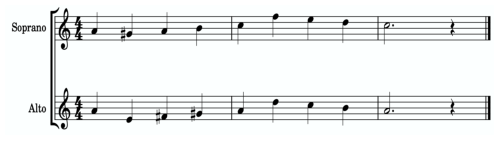
\includegraphics[trim=2.4000000000000004 2.4000000000000004 2.4000000000000004 2.4000000000000004]{pict.pdf}}}
\hspace*{\fill}\\

We would like to bind the sample theme to a name, to make it reusable.  Naming
is not a feature of MuseScore, so we have to annotate a name via embedding Tonart in the
MuseScore Staff Text.  Here is an example showing some standard uses of
Staff Text:

\hspace*{\fill}\\
\raisebox{-0.19999999999999574bp}{\makebox[225.6bp][l]{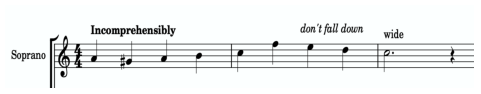
\includegraphics[trim=2.4000000000000004 2.4000000000000004 2.4000000000000004 2.4000000000000004]{pict_2.pdf}}}
\hspace*{\fill}\\

Staff Text in MuseScore is applied to a specific beat.  To translate this
to Tonart, we use the \RktSym{\badlink{\RktValLink{instant}}}\RktMeta{} coordinate.  Text \emph{t} at beat \emph{b} is parsed
as \RktPn{(}\RktSym{\badlink{\RktValLink{@}}}\RktMeta{}\mbox{\hphantom{\Scribtexttt{x}}}\RktMeta{}\RktPn{[}\RktPn{(}\RktSym{\badlink{\RktValLink{instant}}}\RktMeta{}\mbox{\hphantom{\Scribtexttt{x}}}\RktMeta{}\RktSym{b}\RktPn{)}\RktPn{]}\RktMeta{}\mbox{\hphantom{\Scribtexttt{x}}}\RktMeta{}\RktSym{t}\RktPn{)}\RktMeta{}.

However, certain Staff Text applies to a range of music, starting with the beat
the text is on.  For example, {``}\emph{Incomprehensibly}{''} above applies to the
whole passage.  Meanwhile, {``}\emph{wide}{''} applies only to the note.  It is
ambiguous whether {``}\emph{don{'}t fall down}{''} applies to the beat, only, or the
remainder of the passage.  To encode this explicitly, we introduce the
\RktSym{\badlink{\RktValLink{set}}}\RktMeta{} and \RktSym{\badlink{\RktValLink{reset}}}\RktMeta{} notations, as well as the \RktSym{expand{-}set}\RktMeta{}
rewriter, which behave as follows:
\hspace*{\fill}\\
\newcommand{\lam}[2]{\lambda#1.\,#2}

\begin{flushleft}

$\begin{array}{l}
\begin{array}{l}
  (@~[(instant~\mathbf{i})]~(set~\mathbf{e})),\\
  (@~[(instant~\mathbf{j})]~(reset))\\
  \xrightarrow{\hspace*{1cm}\mathbf{expand-set}\hspace*{1cm}}\\
  (@~[(interval~[\mathbf{i}~\mathbf{j}])]~\mathbf{e})\\

  
\end{array}\\[0.1cm]

\end{array}$
\hfill given no $reset$ from $\mathbf{i}$ to $\mathbf{j}$

\end{flushleft}

\hspace*{\fill}\\
Each independent named section of the score module
is punctuated with a MuseScore Section Break.  The Section Break is
interpreted as a \RktSym{\badlink{\RktValLink{reset}}}\RktMeta{} when the score editor score is translated to
Tonart, so that the \RktSym{\badlink{\RktValLink{reset}}}\RktMeta{} does not have to be explicitly specified.
Therefore, forms which apply only to the beat they are attached to can appear
as{-}is, while forms which apply to the rest of the passage are wrapped in
\RktSym{\badlink{\RktValLink{set}}}\RktMeta{}.

We specify the name for the section, as follows:

\hspace*{\fill}\\
\raisebox{-0.7999999999999972bp}{\makebox[232.8bp][l]{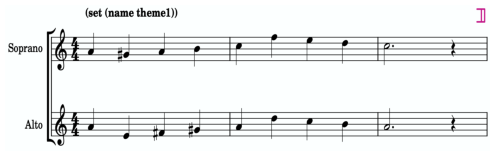
\includegraphics[trim=2.4000000000000004 2.4000000000000004 2.4000000000000004 2.4000000000000004]{pict_3.pdf}}}

(the pink symbol on the top right is MuseScore{'}s indication of a Section Break.)
\hspace*{\fill}\\

To export these names, Racket module syntax goes in the header, as shown:

\hspace*{\fill}\\
\raisebox{-0.3999999999999915bp}{\makebox[232.8bp][l]{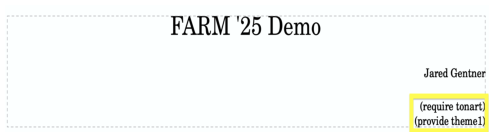
\includegraphics[trim=2.4000000000000004 2.4000000000000004 2.4000000000000004 2.4000000000000004]{pict_4.pdf}}}
\hspace*{\fill}\\

We will only include a couple additional sample sections in this document.
The demo score will include many more.  Here is a section which could
augment the theme with information about where the performers would stand,
presumably in a concert hall setting.

\hspace*{\fill}\\
\raisebox{-0.7999999999999972bp}{\makebox[233.6bp][l]{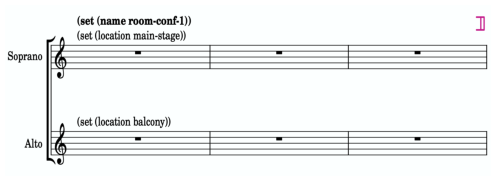
\includegraphics[trim=2.4000000000000004 2.4000000000000004 2.4000000000000004 2.4000000000000004]{pict_5.pdf}}}
\hspace*{\fill}\\

Here is a section which can augment the theme with organ performance information,
allowing it to be performed on an organ at some point in a composition.

\hspace*{\fill}\\
\raisebox{-0.7999999999999972bp}{\makebox[233.6bp][l]{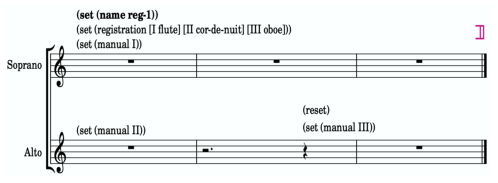
\includegraphics[trim=2.4000000000000004 2.4000000000000004 2.4000000000000004 2.4000000000000004]{pict_6.pdf}}}
\hspace*{\fill}\\

Lastly, here is a section which constructs a canon using the theme.  It also
includes a pedal line, to add some variety.

\hspace*{\fill}\\
\raisebox{-0.3999999999999915bp}{\makebox[234.4bp][l]{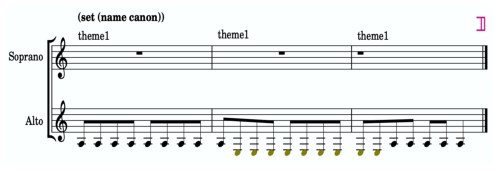
\includegraphics[trim=2.4000000000000004 2.4000000000000004 2.4000000000000004 2.4000000000000004]{pict_7.pdf}}}

\Ssubsection{Transforming to Tonart}{Transforming to Tonart}\label{t:x28part_x22Transformingx5ftox5fTonartx22x29}

Now we would like to translate from MuseScore into Racket and Tonart.  Our
implementation uses MusicXML\Autobibref{~[\hyperref[t:x28autobib_x22Goodx2c_MichaelMusicXMLx3a_An_Internetx2dFriendly_Format_for_Notation_InterchangeIn_Procx2e_Proceedings_of_XML2001httpsx3ax2fx2fwwwx2emusicxmlx2ecomx2fforx2ddevelopersx2fx22x29]{\AutobibLink{5}}]}, as an intermediatary between
the two systems.

Notes are represented in MusicXML like so:

\hspace*{\fill}\\
\raisebox{-0.19999999999998863bp}{\makebox[96.0bp][l]{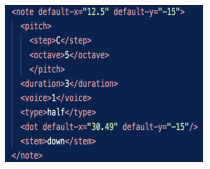
\includegraphics[trim=2.4000000000000004 2.4000000000000004 2.4000000000000004 2.4000000000000004]{pict_8.pdf}}}
\hspace*{\fill}\\

The embeddings are passed through the \RktSym{\badlink{\RktValLink{direction}}}\RktMeta{} element, which is the MusicXML
representation of Staff Text from MuseScore.

\hspace*{\fill}\\
\raisebox{-0.3999999999999986bp}{\makebox[160.0bp][l]{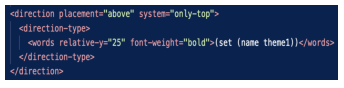
\includegraphics[trim=2.4000000000000004 2.4000000000000004 2.4000000000000004 2.4000000000000004]{pict_9.pdf}}}
\hspace*{\fill}\\

The module system syntax from the header passes through the \RktSym{\badlink{\RktValLink{credit}}}\RktMeta{}
element, which is the MusicXML representation of Composer text, Arranger text, etc.
from MuseScore.

\hspace*{\fill}\\
\raisebox{-0.19999999999999574bp}{\makebox[208.8bp][l]{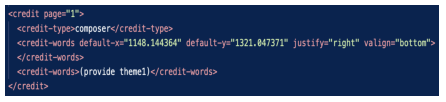
\includegraphics[trim=2.4000000000000004 2.4000000000000004 2.4000000000000004 2.4000000000000004]{pict_10.pdf}}}
\hspace*{\fill}\\

Using Racket{'}s module system and syntax transformers, we are able to turn the
XML file into a Racket module.  We first read the XML at compile time, extracting the
embedded Racket and Tonart code.  To acheive the desired
semantics, we normalize the Tonart code by applying a few rewrites.  First, we
apply \RktSym{expand{-}set}\RktMeta{} to eliminate \RktSym{\badlink{\RktValLink{set}}}\RktMeta{} and \RktSym{\badlink{\RktValLink{reset}}}\RktMeta{}
from the score.  Next, we run a rewriter called \RktSym{\badlink{\RktValLink{instant{-}{\Stttextmore}interval}}}\RktMeta{}, which
gets rid of all remaining \RktSym{\badlink{\RktValLink{instant}}}\RktMeta{} coordinates by translating them into 1 beat
intervals.  Finally, recall that the names we wrote in the score were not
attached using \RktSym{\badlink{\RktValLink{@}}}\RktMeta{}.  In order to get the names correct, we run a
rewriter called \RktSym{attach{-}coordinates}\RktMeta{}, which takes unattached coordinates
that are written in a score, and attaches them to notations , using the following
rule:
\hspace*{\fill}\\
\newcommand{\lam}[2]{\lambda#1.\,#2}

\begin{flushleft}

$\begin{array}{l}
\begin{array}{l}
  (@~[\mathbf{C}~...]~\mathbf{c}),\\
  (@~[\mathbf{E}~...]~\mathbf{e})\\
  \xrightarrow{\hspace*{0.1cm}\mathbf{(attach-coordinates)}\hspace*{0.1cm}}\\
  (@~[\mathbf{E}~...~\mathbf{c}]~\mathbf{e})\\

  
\end{array}\\[0.1cm]

\end{array}$

\end{flushleft}
given $\mathbf{c}$ is a coordinate and $\mathbf{E }$ is within $\mathbf{C}$

\hspace*{\fill}\\

After applying this rewrite, our notations now have their respective names attached.

Following these rewrites, the final step is to realize the named notations into Racket definitions.
This is done using the realizer \RktSym{\badlink{\RktValLink{namespace{-}define{-}realizer}}}\RktMeta{}.  This realizer takes a score with
named notations, and turns it into a series of Racket definitions.

For each set of notations \emph{N} ... with attached name \emph{n}, the realizer
generates one Racket define form, \RktPn{(}\RktSym{\badlink{\RktValLink{define{-}art}}}\RktMeta{}\mbox{\hphantom{\Scribtexttt{x}}}\RktMeta{}\RktSym{\badlink{\RktValLink{n}}}\RktMeta{}\mbox{\hphantom{\Scribtexttt{x}}}\RktMeta{}\RktSym{N}\RktMeta{}\mbox{\hphantom{\Scribtexttt{x}}}\RktMeta{}\RktSym{{\hbox{\texttt{.}}}{\hbox{\texttt{.}}}{\hbox{\texttt{.}}}}\RktPn{)}\RktMeta{}.
\RktSym{\badlink{\RktValLink{define{-}art}}}\RktMeta{} defines a Racket binding which can be used in embedded Tonart
programs.  These definitions are combined with the module system statements from
the score editor score, completing the translation.

After requiring the score module, we can use the bindings from the score editor
score.  Here is a rendering of the sample theme composed with the location
configuration using the Tonart \RktSym{\badlink{\RktValLink{staff{-}realizer}}}\RktMeta{}.

\begin{SCodeFlow}\begin{RktBlk}\begin{SingleColumn}\begin{RktBlk}\begin{SingleColumn}\RktPn{(}\RktSym{\badlink{\RktValLink{realize}}}\mbox{\hphantom{\Scribtexttt{x}}}\RktPn{(}\RktSym{\badlink{\RktValLink{staff{-}realizer}}}\RktPn{)}

\mbox{\hphantom{\Scribtexttt{xx}}}\RktSym{theme1}\mbox{\hphantom{\Scribtexttt{x}}}\RktSym{room{-}conf{-}1}\RktPn{)}\end{SingleColumn}\end{RktBlk}

\raisebox{-0.0bp}{\makebox[213.6bp][l]{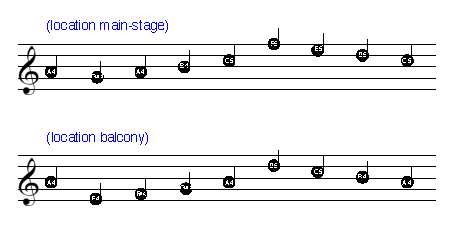
\includegraphics[trim=2.4000000000000004 2.4000000000000004 2.4000000000000004 2.4000000000000004]{pict_11.pdf}}}\end{SingleColumn}\end{RktBlk}\end{SCodeFlow}

\Ssubsection{Finale}{Finale}\label{t:x28part_x22Finalex22x29}

For the remainder of the demo, an environment featuring prepared MuseScore and
text modules will be showcased.  The scores will be written in the demo
language, and the showcase will be a small improvisatory performance achieved by
writing Tonart in a REPL environment, with the demo environment loaded.

\Ssubsection{Limitations and Future Directions}{Limitations and Future Directions}\label{t:x28part_x22Limitationsx5fandx5fFuturex5fDirectionsx22x29}

While embedding into an existing score editor is great
for accesibility, it still leaves much to be desired vis{-}\`{a}{-}vis interoperation
between host language and embedded language.  The score editor score can only be
loaded as a module, not embedded directly inside other code.  Moreover, it seems
impossible to report errors on the original syntax, as, in our case, MuseScore
and Racket have no means to communicate such error reporting information with
each other.  Finally, the extra intermediary form of MusicXML can be a hassle
to manage\Footnote{\FootnoteRef{\textsuper{\hyperref[t:x28x7ccounterx2dx28x29x7c_x23x28structx3ageneratedx2dtagx29x29]{1}}}\FootnoteContent{In the current implementation, many errors are actually reported
with source locations coming from \emph{inside the MusicXML}. This is somewhat
impressive, but misses the mark from a useability perspective.}}

\Ssubsubsection{Interactive Visual Syntax}{Interactive Visual Syntax}\label{t:x28part_x22Interactivex5fVisualx5fSyntaxx22x29}

Interactive visual syntax\Autobibref{~[\hyperref[t:x28autobib_x22Andersenx2c_Leifx2c_Ballantynex2c_Michaelx2c_and_Felleisenx2c_MatthiasAdding_interactive_visual_syntax_to_textual_codeIn_Procx2e_ACM_on_Programming_Languagesx2c_ppx2e_1x2dx2d282020httpsx3ax2fx2fdoix2eorgx2f10x2e1145x2f3428290x22x29]{\AutobibLink{3}}]} allows for creating interactive,
embeddable graphical elements that still manage to leverage the bindings and
scope of the host language, just as successful textual embeddings do.  Visual
Syntax additionally provides a mechanism for graphically reporting errors.  On
the one hand, integrating with an existing score editor is appealing, by
enabling existing workflows and reusing years of score editor specific work done
by others.  On the other hand, a bespoke visual syntax or syntaxes would be a
powerful tool for providing that familiar interface, while retaining the
benefits of a textual embedding, and getting rid of intermediate
representations.

\Ssubsubsection{Output{-}Directed Programming}{Output{-}Directed Programming}\label{t:x28part_x22Outputx2dDirectedx5fProgrammingx22x29}

In creating the translation from MuseScore to Tonart, we ended up implicitly
defining a relation between elements of the MuseScore score and Tonart
notations.  Output{-}Directed Programming uses this relation in both directions
and in a live fashion.  \emph{Sketch{-}n{-}Sketch}\Autobibref{~[\hyperref[t:x28autobib_x22Hempelx2c_Brianx2c_Lubinx2c_Justinx2c_and_Chughx2c_RaviSketchx2dnx2dSketchx3a_Outputx2dDirected_Programming_for_SVGIn_Procx2e_32nd_Annual_ACM_Symposium_on_User_Interface_Software_and_Technologyx2c_ppx2e_281x2dx2d2922019httpsx3ax2fx2fdoix2eorgx2f10x2e1145x2f3332165x2e3347925x22x29]{\AutobibLink{1}}]} is an
Output{-}Directed editor for SVGs.  It allows both graphical and
textual editing.  Edits to the grahpic reflect immediately in the graphic{'}s
domain{-}specific source code, and edits to the source code immediately reflect on
the graphic.  It is once again hard to imagine such a technology working with an
existing score editor.  That does not change the fact that an Output{-}Directed
music editor would minimize intermediate representations, maximize feedback, and
be capable of providing well{-}correlated graphical error messages.\label{t:x28part_x28gentag_4x29x29}

\begin{FootnoteBlock}\FootnoteBlockContent{\FootnoteTarget{\textsuper{\label{t:x28x7ccounterx2dx28x29x7c_x28gentag_5x29x29}\textsf{1}}}In the current implementation, many errors are actually reported
with source locations coming from \emph{inside the MusicXML}. This is somewhat
impressive, but misses the mark from a useability perspective.}\end{FootnoteBlock}

\sectionNewpage

\Ssectionstarx{References}{References}\label{t:x28part_x22docx2dbibliographyx22x29}

\begin{bigtabular}{@{\bigtableleftpad}l@{}l@{}}
\hbox{\Autocolbibnumber{[1]}} &
\hbox{\Autobibtarget{\label{t:x28autobib_x22Hempelx2c_Brianx2c_Lubinx2c_Justinx2c_and_Chughx2c_RaviSketchx2dnx2dSketchx3a_Outputx2dDirected_Programming_for_SVGIn_Procx2e_32nd_Annual_ACM_Symposium_on_User_Interface_Software_and_Technologyx2c_ppx2e_281x2dx2d2922019httpsx3ax2fx2fdoix2eorgx2f10x2e1145x2f3332165x2e3347925x22x29}\Autocolbibentry{Hempel, Brian, Lubin, Justin, and Chugh, Ravi. Sketch{-}n{-}Sketch: Output{-}Directed Programming for SVG. In \textit{Proc. 32nd Annual ACM Symposium on User Interface Software and Technology}, pp. 281{--}292, 2019. \href{https://doi.org/10.1145/3332165.3347925}{\Snolinkurl{https://doi.org/10.1145/3332165.3347925}}}}} \\
\hbox{\Autocolbibnumber{[2]}} &
\hbox{\Autobibtarget{\label{t:x28autobib_x22Gentnerx2c_JaredDemox3a_Composable_Compositions_with_TonartIn_Procx2e_12th_ACM_SIGPLAN_International_Workshop_on_Functional_Artx2c_Musicx2c_Modellingx2c_and_Designx2c_ppx2e_42x2dx2d442024httpsx3ax2fx2fdoix2eorgx2f10x2e1145x2f3677996x2e3678294x22x29}\Autocolbibentry{Gentner, Jared. Demo: Composable Compositions with Tonart. In \textit{Proc. 12th ACM SIGPLAN International Workshop on Functional Art, Music, Modelling, and Design}, pp. 42{--}44, 2024. \href{https://doi.org/10.1145/3677996.3678294}{\Snolinkurl{https://doi.org/10.1145/3677996.3678294}}}}} \\
\hbox{\Autocolbibnumber{[3]}} &
\hbox{\Autobibtarget{\label{t:x28autobib_x22Andersenx2c_Leifx2c_Ballantynex2c_Michaelx2c_and_Felleisenx2c_MatthiasAdding_interactive_visual_syntax_to_textual_codeIn_Procx2e_ACM_on_Programming_Languagesx2c_ppx2e_1x2dx2d282020httpsx3ax2fx2fdoix2eorgx2f10x2e1145x2f3428290x22x29}\Autocolbibentry{Andersen, Leif, Ballantyne, Michael, and Felleisen, Matthias. Adding interactive visual syntax to textual code. In \textit{Proc. ACM on Programming Languages}, pp. 1{--}28, 2020. \href{https://doi.org/10.1145/3428290}{\Snolinkurl{https://doi.org/10.1145/3428290}}}}} \\
\hbox{\Autocolbibnumber{[4]}} &
\hbox{\Autobibtarget{\label{t:x28autobib_x22Flattx2c_MatthewComposable_and_Compilable_Macrosx3a_You_Want_it_Whenx3fIn_Procx2e_ACM_Intlx2e_Confx2e_Functional_Programmingx2c_ppx2e_72x2dx2d832002x22x29}\Autocolbibentry{Flatt, Matthew. Composable and Compilable Macros: You Want it When? In \textit{Proc. ACM Intl. Conf. Functional Programming}, pp. 72{--}83, 2002.}}} \\
\hbox{\Autocolbibnumber{[5]}} &
\hbox{\Autobibtarget{\label{t:x28autobib_x22Goodx2c_MichaelMusicXMLx3a_An_Internetx2dFriendly_Format_for_Notation_InterchangeIn_Procx2e_Proceedings_of_XML2001httpsx3ax2fx2fwwwx2emusicxmlx2ecomx2fforx2ddevelopersx2fx22x29}\Autocolbibentry{Good, Michael. MusicXML: An Internet{-}Friendly Format for Notation Interchange. In \textit{Proc. Proceedings of XML}, 2001. \href{https://www.musicxml.com/for-developers/}{\Snolinkurl{https://www.musicxml.com/for-developers/}}}}}\end{bigtabular}

\postDoc
\end{document}
